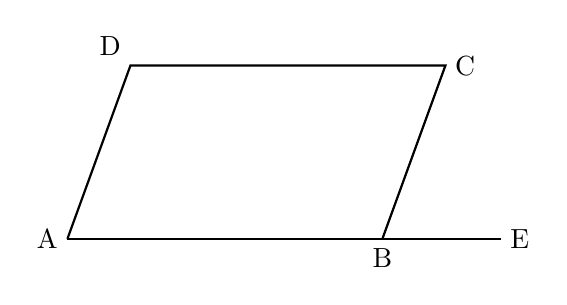
\begin{tikzpicture}[scale=1]

    % Define the coordinates for the parallelogram and the extended line
    % Proportions are matched to the provided image
    \coordinate (A) at (0,0);
    \coordinate (B) at (4,0);
    \coordinate (E) at (5.5,0);
    \coordinate (C) at (4.8,2.2);
    \coordinate (D) at (0.8,2.2);

    % Draw the base line extending from A through B to E
    \draw[thick] (A) -- (E);

    % Draw the remaining sides of the parallelogram ABCD
    \draw[thick] (A) -- (D) -- (C) -- (B);

    % Place the labels for the points exactly where they appear in the image
    \node[left] at (A) {A};
    \node[below] at (B) {B};
    \node[right] at (C) {C};
    \node[above left] at (D) {D};
    \node[right] at (E) {E};

\end{tikzpicture}